\noindent V Altiu byla vytvořena DPS pro DP 4. řádu, PP 2. řádu. Keramický vícevrstvý kapacitor byl zvolen vhodný pro pro povrchovou montáž plošných spojů (SMD) typ C0402C100K56ACAUTO (10~pF, jmenovité napětí stejnosměrného proudu 50~V, tolerance 10~\%). Symboly a footprinty k LM13700M a kapacitoru byly staženy ze~ \url{snapeda.com}. \\
\\
Jako zdroj proudu lze použít NPN tranzistor, nebo operační zesilovač. Různé přístupy k řízení OTA vstupním proudem pomocí napěťového zdroje jsou popsány na obrázku \ref{s:DC} (Geiger, Sanchez-Sinencio \cite{25}). Obrázek a) je nejjednodušší zapojení, ale toto zapojení je velmi citilivé na malé změny napětí. V zapojení b) je řídící napětí uzemněno, ale $V_c$ je citlivé na změny napětí mezi bází a emitorem tranzistoru a na úbytek napětí na diodě. V zapojení c) je řídící napětí také uzemněno a není závislé na součtu nebo vyrušení napětí na pn přechodech. Zenerova dioda je použita k udržení napětí. Frekvenční odezva OZ se zde neuvažuje, protože máme stejnosměrné napětí. Všechna zapojení jsou velmi citlivá na malé změny $V_c$. \\
\\
K řízení odporu byl použit trimmer o hodnotě odporu 1~M$\Omega$. Zapojení se zdrojem na 1~V odpovídá klidový stejnosměrný pracovní proud 1~$\mu$A, který odpovídá dvojnásobku proudu použitého v simulaci. Dle dokumentace k simulačnímu bloku LM13700 je reálný proud dvakrát větší. Trimmer byl zvolen 3361S-1-105GLF (tolerance 10~\%, jmenovitý výkon 500~mW). Schematická značka a footprint s rozměry převzatými z dokumentace byly vytvořeny v Altiu.
\begin{figure}[h]
\centering
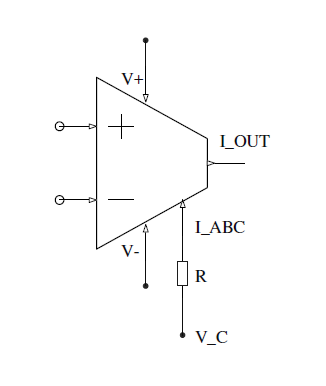
\includegraphics[scale=0.5]{current.png}
\caption{Schéma zapojení napěťového zdroje pro klidový stejnosměrný pracovní proud \label{s:DC}}
\end{figure}
\begin{figure}[h]
\centering
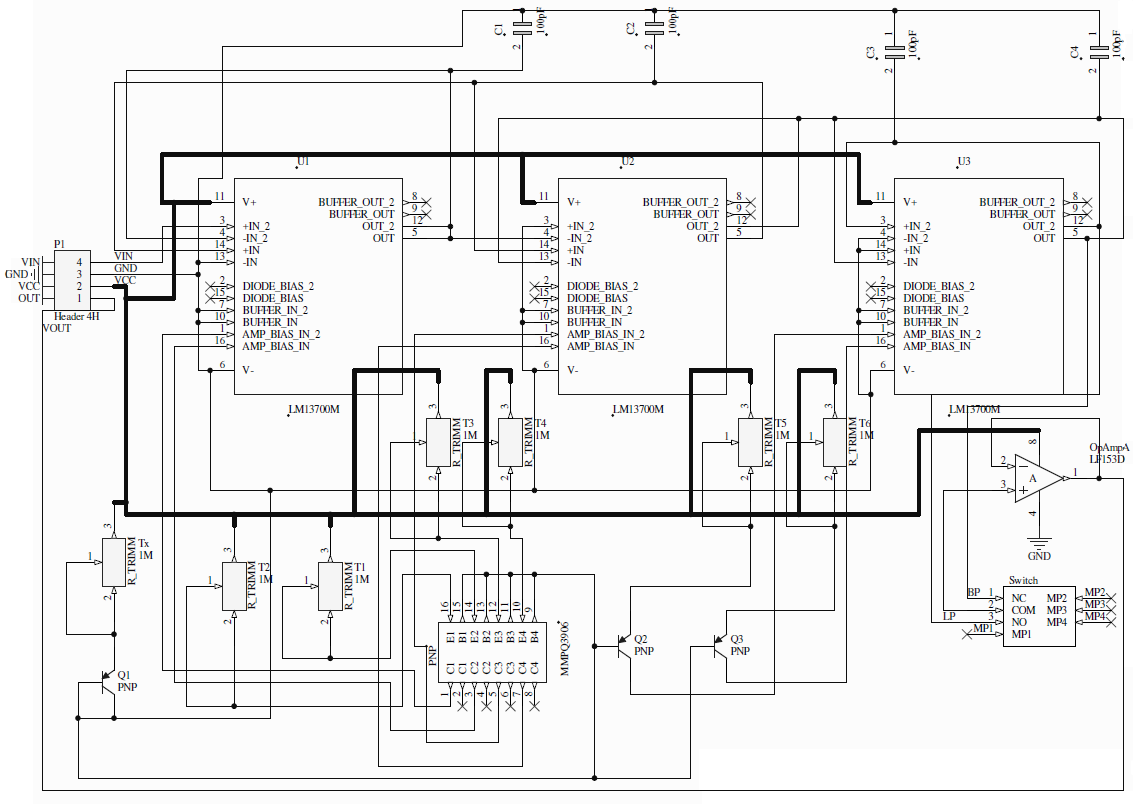
\includegraphics[scale=0.5]{altium.png}
\caption{Schéma obvodu v Altiu}
\end{figure}
\begin{figure}[h]
\centering
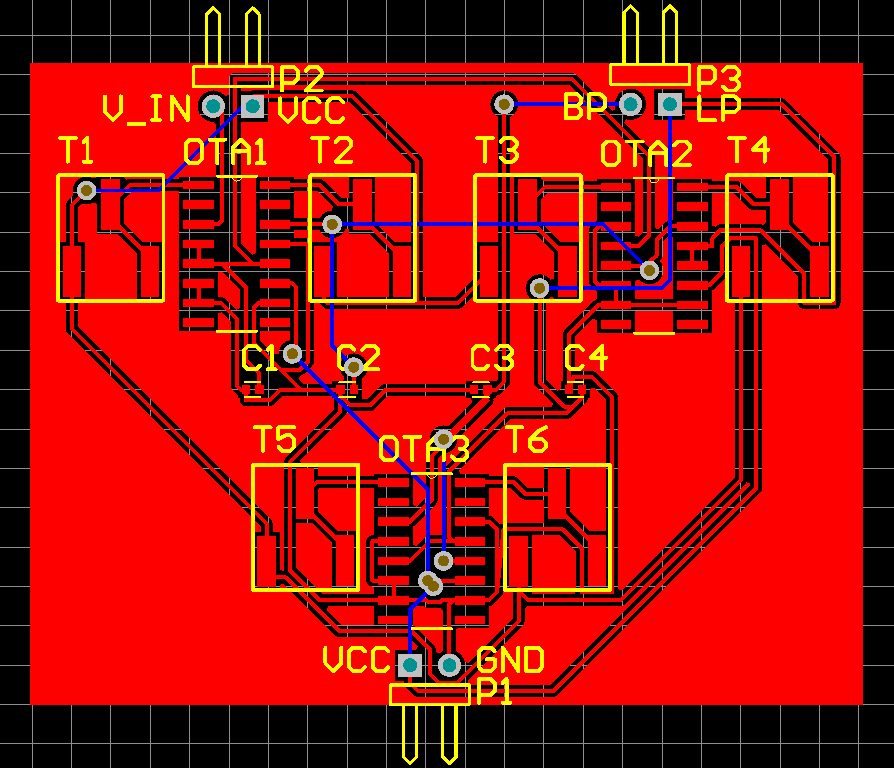
\includegraphics[scale=0.5]{altium2.png}
\caption{PCB layout}
\end{figure}